\subsubsection{Kinematics}
The Kamikaze's movement underwater may be one of the most important aspects of
the design. We had to ensure stability, maneuverability, and speed. We achieved
this by focusing on two main aspects:
\begin{itemize}
        
    \item \textbf{Thrusters Configuration:} We employed a seventh thruster this year to
        improve the robot's maneuverability. With the current vectored thrusters
        configuration and this new thruster, we can achieve motion in 6 degrees of freedom.
        This novel configuration may be the first of its kind to allow for such a wide range of motion while only using 7 thrusters.

        \item \textbf{PID Control:} We have implemented PID controllers for all critical movement axes, allowing for
        precise control over the robot's movement and ensures that it remains stable in the water. We implemented an FFT (Fast Fourier Transform)
        based auto-tuning algorithm to tune the PID parameters, as this is our first year using the new Vehicle. We also supplemented the algorithm with a live
        plotting feature, shown in figure \ref{fig:pid_live},
         to allow for manual adjustments to the PID parameters.
\end{itemize}
\begin{figure}[h]
    \centering
    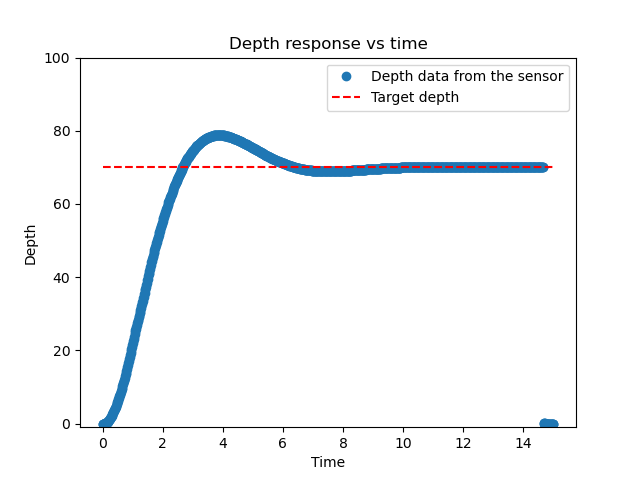
\includegraphics[width=0.5\textwidth]{Sections/3Design&Manufacturing/tex/Software/images/Pid.png}
    \caption{Live Plotting of PID Parameters}
    \label{fig:pid_live}
\end{figure}

\subsection{Open Sourcing the Kamikaze}
We have all of our working code available on our GitHub repository. A lot of effort
was made this year to maintain, document, and clean up the code, making it easier
for future teams to understand and build upon. We believe that this is a crucial
step in the development of the Kamikaze, as it allows for a more collaborative
environment and ensures that the knowledge gained from each year is not lost. 

